\section{Methodology and Implementation}
% What were the methods used?
% How was the problem designed?
% Driving concepts
% Equations
% Figures

A modular, agent-based is an ideal approach for solving complicated
physics-dependent supply chain problems involving material routing, facility
deployment, regional and institutional hierarchies.

\subsection{Framework Structure}
% (OO, cpp, xml, backends, inheritances, mixins, generic apis, etc.)

Agent-based modeling is inherently object oriented. 

The core of the simulator creates a set of key classes on which agent plugins 
are based. In addtion, a set of key tools are also provided, to enrich the API 
and provide a robust suite of behaviors for the developer.

<diagram of core, modules, toolkit, etc>

Agent plug-ins utilize the generic core API to interact with one another. 
Mainly they do this by trading resources. 

<diagram of black box facilities>

\subsection{Cluster-Ready Software}

Because this doesn't rely on PowerSim, GoldSim, Excel, or any other COTS 
Windows-based software, we can run singular instances of Cyclus 
on large linux machines that have lots more capability than hacked together 
Windows clusters. 

\subsection{Dynamically loadable libraries}
% (diagram)

A key innovation that has previously not been implemented in nuclear fuel cycle 
simulators in the literature is implementing this generic API and modular 
architecture into a suite of dynamically loadable ``plug-in'' libraries. 

This approach allows contribution to an ecosystem of libraries. The 
scientist-developer can therefore focus on generating a model within their 
sphere of expertise, while relying on the model contributions of others to fill 
in the other technologies.

This is implemented largely through a clean API and a modern build system.

Additionally, the clean plug-in architecture loads modules without any
modifications to the \Cyclus kernel. Thus, as in Figure \ref{fig:modifiedopen},
closed-source archetypes can be used with the simulator alongside open-source
archetypes. This architecture therefore allows closed-source libraries (e.g.,
those representing sensitive nuclear processes and subject to export control)
to be developed and used privately.

\begin{figure}[htbp!]
\begin{center}
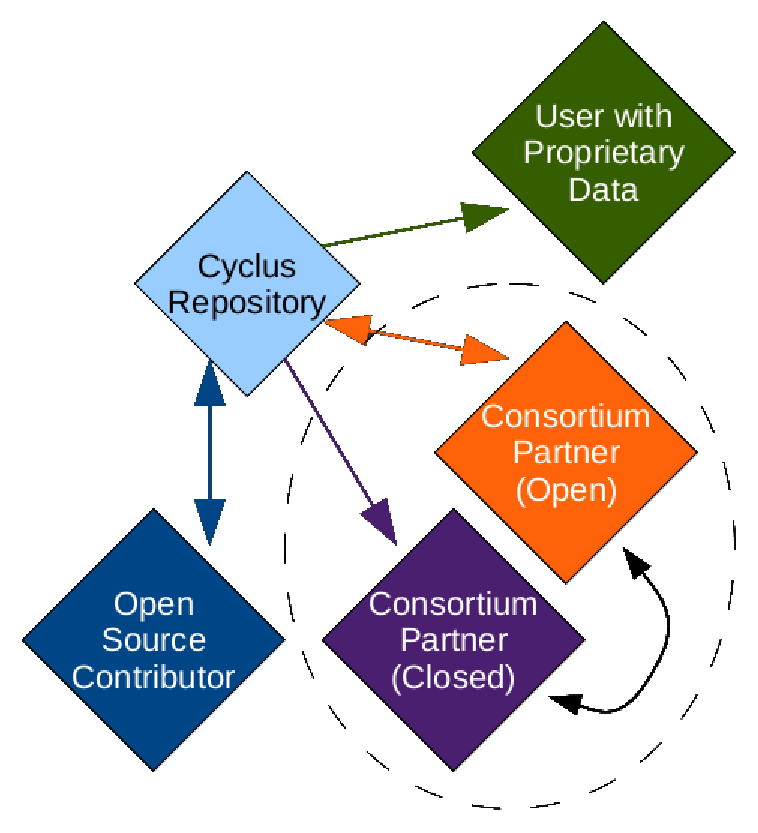
\includegraphics{./images/modifiedopen.eps}
\end{center}
\caption{The \Cyclus framework enables fully open, partially open, and fully
closed collaborations.}
\label{fig:modifiedopen}
\end{figure}


\subsection{Agent Interchangability}
% interchangeability due to exchange behavior api

This approach enables ``apples-to-apples'' comparisons, something that has been 
sorely missing in previous simulators.

By making the facilities interchangeable, it combinatorically increases the 
number of scenarios that can be modeled. The user can choose to model just the 
front end or just the back end of a fuel cycle. 

This is implemented with an API that focuses on treating the agents as black 
boxes. 

\subsection{Region/Institution/Facility hierarchy}
% (diagram)

Cyclus has three core agent classes that be subclassed to create a simulation
archetype: Region, Institution, and Facility. At present, Regions, Institutions,
and Facilities (RIF) conceptually form a nested structure in a Cyclus simulation,
i.e., Facilities exist in (i.e., are managed by) Institutions and Institutions
exist in Regions.

Importantly, the RIF separation allows for preferential trading. For example,
Facilities in the same Institution can preferentially trade with each
other. Similarly, Regions can be given a location proxy, and the trade between
Facilities can be informed by their regional proximity.

\subsection{Discrete Object Tracking}
% Resources, Materials (note isotope tracking, decay behavior)

Discrete facility and material tracking is more realistic an dmore 

\subsection{Toolkit}
% library of tools
% contributions to the toolkit
% place for metrics

The toolkit is a place for developers and users to contribute common-use tools 
for calculating metrics, managing process physics, and handling data.

This was implemented by liberal use of namespaces and is populated with an
introductory suite of useful tools, including helper classes for managing
facility deployment, minimum cost facility deployment decision making, and for
enrichment-related calculations.

\subsection{Cycamore}
% base modules

Cycamore contains a number of useful facility models that are a mere base-set.
Additional modules are needed for interesting fuel cycle simulation. However,
simple, once-through fuel cycles can be generated with Cycamore and Cyclus alone.

<diagram of a possible Cycamore-only simulation>
